\subsection{Quantum FDTD (QFDTD)}
\label{section:tools:qfdtd}


One model proposed to explain the high charge states seen in some experiments
is the lowering of the ionization barrier, used in conjunction with classical
MD simulations. This model assumes that an electron can be ionized when
the potential of a neighbouring ion lowers the potential of the electron's
parent ion - this is called "Barrier Lowering"~\cite{Georgescu2007,Fennel2010}.
An open question is how close this model, used
with a classical MD, is to reality. Special care needs to be taken when a
particle, evolving in a quantum world, is to be treated classically.
How does
the bound electron's wavefunction react to the presence of a second ion
perturbing the potential? How can the $U_b$ approximation to the cluster
environment, described in chapter~\ref{section:intro:Vb}, be tested?
Is the wavefunction really evolving into a state
where we can say the electron is shared by the two ions? If the electron is
really shared by the two ions, can we classically let it evolve inside the
cluster environment?

These questions pushed us to look at the quantum aspects in more detail. Many
tools exist to calculate the ground state of a system, even with
multiple electrons (with different levels of approximations),
as described previously. Additionally, excited states are
capital in ACI and as such we needed a tool that could give us information not
only on the ground state but also on excited states.

After stumbling on an interesting article that used the Finite-Difference
Time-Domain (FDTD) algorithm to solve \schrodinger equation~\cite{Sudiarta2007}
it was decided to explore this idea since not much work could be found on this
\textit{Quantum FDTD} (QFDTD) method and beceause of previous experiences
implementing electrodynamics FDTD.

FDTD is an established algorithm developed in 1966 by Yee~\cite{Yee1966} to solve
Maxwell's equation on a grid using leap-frog integration.
It is actually the method used in PIC simulations to propagate the electromagnetic
field through the grid.
The number of
scientific articles using FDTD has exponentially increased since the '80s
largely due to the increase in computational resources. Indeed, a three
dimensional grid with the three vector components of both the electric and
magnetic fields requires huge amount of memory that was definitely not present
in the late '60s. The reader is invited to read the excellent book on FDTD by
Allen Taflove and Susan Hagness~\cite{Taflove2005} covering 40 years of FDTD
development in electrodynamics simulations.

Other simulation techniques like Finite-Element Methods (FEM) or Finite-Volume
Methods (FVM) can be seen as more complex than Finite-Differences Methods
(FDM). This gives some elegance and simplicity to the FDM algorithms.
Additionally, since FDTD is an explicit algorithm, implementations are
generally easy and efficient and the local nature of the algorithm makes it
easily parallelizable on distributed memory systems.

Sullivan was the first to apply the FDTD method to solve the \schrodinger
equation in his 2000 book~\cite{Sullivan2000} where he obtains the wavefunction
of an electron hitting a potential barrier in one dimension.
Later, in 2001, he used the FDTD
method to simulate one and two electrons in a quantum dot~\cite{Sullivan2001}.
The Hartree-Fock approximation was used to describe the two electrons problem
and thus required the use of Fourier transforms to calculate the Coulomb
and exchange terms. Due to this additional calculation, the problem was
restricted to two dimensions only. The following year, he introduced a method
to calculate the eigenstates of an arbitrary system using
FDTD~\cite{Sullivan2002}. This method requires two distinct simulations: the
first one finds the eigenvalues and the second one stores the states
corresponding to these eigenvalues, doubling the simulation time required.
The interaction with a magnetic field was included through the vector potential
and later~\cite{Sullivan2003,Sullivan2004} used to calculate spin interaction.
Only in 2005 were the first three dimensional
simulations~\cite{Sullivan2005a} performed as proof of concept; only a
single electron was simulated. Eigenstates and eigenvalues were obtained for a
simple quantum well in addition as a two ions system. A more complicated three
dimensional system was later simulated in~\cite{Sullivan2005b}, still with a
single electron.

Later Sudiarta suggested~\cite{Sudiarta2007} a new way to use the FDTD method to
solve the \schrodinger equation for a single electron system. By switching to
\textit{imaginary time}, \schrodinger equation can be solved more easily and
more efficiently to get the eigenvalues and eigenstates of the system. It was
later shown that the interaction with a magnetic field could also be added to
the imaginary-time method~\cite{Sudiarta2008} and that FDTD could be used to
construct the thermal density matrix of a single particle~\cite{Sudiarta2009}.
Strickland \textit{et al.} parallelized the method~\cite{Strickland2010} and
even released its code through the GPL v2
license\footnote{\url{http://sourceforge.net/projects/quantumfdtd}}.


Both real-time and imaginary-time methods were implemented for this thesis. The
two algorithms are described as follows.


\subsubsection{Real time}

First, let's define the time dependent \schrodinger equation describing a
wavefunction $\psi$ inside a potential $V$:
\begin{align}
\im \hbar \delt{  } \ket{\psi\pa{\vr, t}}
    & = \pa{-\frac{\hbar^2}{2 m} \laplacian{} + V\pa{\vr, t} } \ket{\psi\pa{\vr,
t}}.
\label{eqn:schrodinger:si}
\end{align}
To ease the calculation, let's switch to atomic units where $\hbar = 1$, $m
= 1$ and $e_0 = 1$:
\begin{align}
\im \delt{  } \ket{\psi\pa{\vr, t}}
    & = \pa{-\frac{1}{2} \laplacian{} + V\pa{\vr, t} } \ket{\psi\pa{\vr, t}}.
\label{eqn:schrodinger:au}
\end{align}
At initial time $t = 0$, the wavefunction $\ket{\psi\pa{\vr, t}}$ is
decomposed into its eigenstates basis:
\begin{align}
\ket{\psi\pa{\vr, t=0}} & = \sum_{n=0}^{\infty} c_n \ket{\phi_n\pa{\vr}}.
\label{eqn:wavefunction:real:initial}
\end{align}
The time-evolution operator (or propagator) $\oU\pa{t}$ is, in atomic units:
\begin{align}
\oU\pa{t} & = \ex{ - \im t \oH },
\label{eqn:propagator:real}
\end{align}
and when applied to the initial state~\eqref{eqn:wavefunction:real:initial}
gives the time evolution of the wavefunction:
\begin{align}
\oU\pa{t} \ket{\psi\pa{\vr, t=0}}
    = \ket{\psi\pa{\vr, t}}
  & = \e{ - \im t \oH } \sum_{n=0}^{\infty} c_n \ket{\phi_n\pa{\vr}}.
\end{align}
Since the operator $\oH$ applied to the eigenstates
$\ket{\phi_n\pa{\vr}}$ gives the eigenvalues $E_n$, the previous equation
becomes:
\begin{align}
\ket{\psi\pa{\vr, t}}
 & = \sum_{n=0}^{\infty} \e{ - \im t E_n } c_n \ket{\phi_n\pa{\vr}}.
\label{eqn:wavefunction:eigenstates:time_evolution:real}
\end{align}
The time evolution of each eigenstates is thus an oscillation between their real
and imaginary parts of which the frequency is given by the eigenvalue $E_n$.



Equation~\eqref{eqn:schrodinger:au} can now be solved either in real-time or
imaginary-time, the former being explained first.

Let's separate the real and imaginary components of equation
\eqref{eqn:schrodinger:au} (and simplifying the notation):
\begin{align}
\im \delt{  } \pa{ \psi_R + \im \psi_I}
    & = \pa{-\frac{1}{2} \laplacian{} + V }
        \pa{ \psi_R + \im \psi_I},
% \\
% \im \delt{  } \psi_R - \delt{  } \psi_I
%     & = \pa{-\frac{1}{2} \laplacian{} + V } \psi_R
%       + \im \pa{-\frac{1}{2} \laplacian{} + V } \psi_I
\end{align}
giving two equations describing the time evolution of two effective fields:
\begin{subequations}
\begin{align}
\delt{  } \psi_R & =   \pa{-\frac{1}{2} \laplacian{} + V } \psi_I,
\label{eqn:schrodinger:real:real} \\
\delt{  } \psi_I & = - \pa{-\frac{1}{2} \laplacian{} + V } \psi_R.
\label{eqn:schrodinger:real:imag}
\end{align}
\label{eqn:schrodinger:real}
\end{subequations}
The real and imaginary parts in equation~\eqref{eqn:schrodinger:real} can be
compared to the electric and magnetic fields in the traditional electrodynamics
FDTD method. The integration is performed using a leap-frog scheme. We
first define $\psi_{i,j,k}^{n}$ the wavefunction located at the grid cell
$\pa{i,j,k}$ and at time step~$n$. Then equation
\eqref{eqn:schrodinger:real:imag} is evaluated at time step~$n$ and, using
(second order) central-differences, we get:
\begin{align}
\left. \delt{  } \psi_I \right|_{n}
& = \left. - \pa{-\frac{1}{2} \laplacian{} + V^{n} } \psi_R \right|_{n}, \\
\frac{\psi_{I}^{n+1/2} - \psi_{I}^{n-1/2}}{\Delta t}
& = - \pa{-\frac{1}{2} \laplacian{} + V^{n} } \psi_{R}^{n}, \\
\psi_{I}^{n+1/2}
& = \psi_{I}^{n-1/2} - \Delta t \pa{-\frac{1}{2} \laplacian{} + V^{n} }
\psi_{R}^{n}.
\label{eqn:schrodinger:real:imag:discretized}
\end{align}
Similarly, defining the time derivative in~\eqref{eqn:schrodinger:real:real} at
time step~$n$ and again using (second order) central-differences:
\begin{align}
\left. \delt{  } \psi_R \right|_{n+1/2}
& = \left. \pa{-\frac{1}{2} \laplacian{} + V^{n} } \psi_I \right|_{n+1/2}, \\
\frac{\psi_{R}^{n+1} - \psi_{R}^{n}}{\Delta t}
& = \pa{-\frac{1}{2} \laplacian{} + V^{n} } \psi_{I}^{n+1/2}. \\
\psi_{R}^{n+1}
& = \psi_{R}^{n} + \Delta t \pa{-\frac{1}{2} \laplacian{} + V^{n} }
\psi_{I}^{n+1/2},
\label{eqn:schrodinger:real:real:discretized}
\end{align}

Lastly, the Laplacian is discretized on a grid using (second order)
central-differences:
\begin{align}
\laplacian{} \psi_{i,j,k}^{n} \approx
      \frac{ \psi_{i+1,j,k}^{n} - \psi_{i-1,j,k}^{n} }{2 \Delta x}
    + \frac{ \psi_{i,j+1,k}^{n} - \psi_{i,j-1,k}^{n} }{2 \Delta y}
    + \frac{ \psi_{i,j,k+1}^{n} - \psi_{i,j,k-1}^{n} }{2 \Delta z}.
\label{eqn:laplacian:discretized}
\end{align}

Equations~\eqref{eqn:schrodinger:real:imag:discretized},
\eqref{eqn:schrodinger:real:real:discretized} and
\eqref{eqn:laplacian:discretized} are then used to propagate in time the real
and imaginary components of the electronic wavefunction. Note that, contrary
to the Yee cell in the electrodynamics FDTD, the two components of the
wavefunction do not have to be defined at different location inside the grid
cell; they are defined at the same locations as shown in figure
\ref{fig:qfdtd:cell}.

\begin{figure}
 \centering
    \begin{subfigure}{0.48\columnwidth}
        \centering
        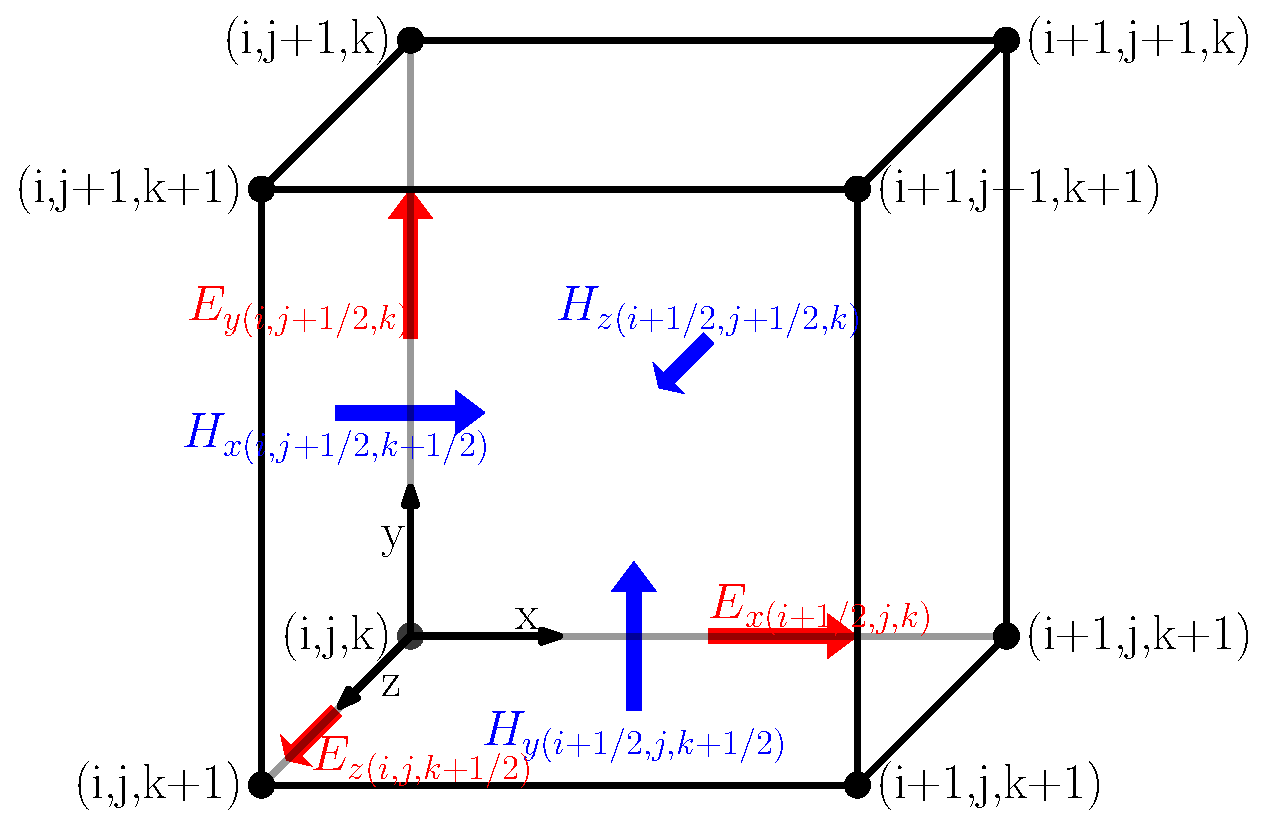
\includegraphics[width=\textwidth]{figures/fdtd_cell_yee}
        \caption{Yee cell}
        \label{fig:qfdtd:cell:yee}
    \end{subfigure}
    \begin{subfigure}{0.48\columnwidth}
        \centering
        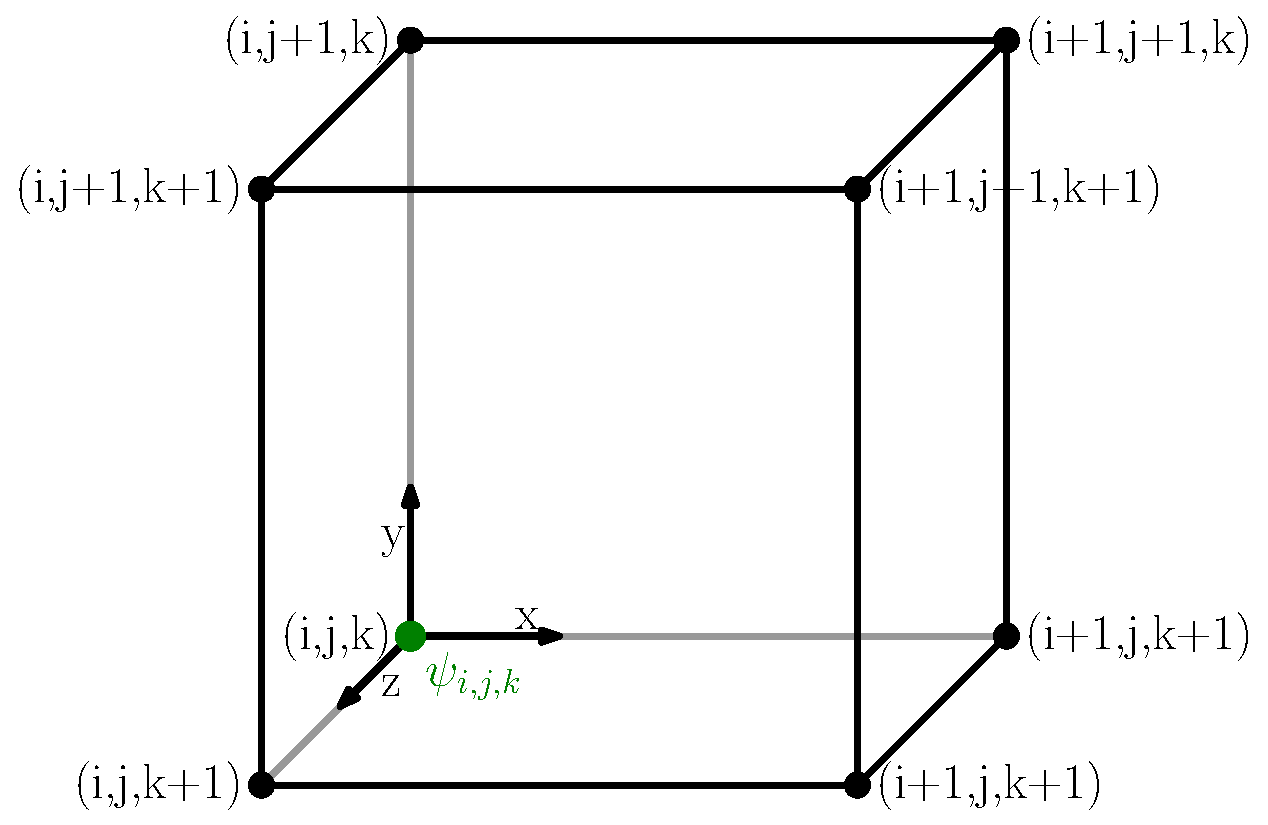
\includegraphics[width=\textwidth]{figures/fdtd_cell_qfdtd}
        \caption{QFDTD cell}
        \label{fig:qfdtd:cell:qfdtd}
    \end{subfigure}
        \caption{\label{fig:qfdtd:cell}Yee cell used in electrodynamic FDTD vs QFDTD
        cell with id $\pa{i,j,k}$. Other vertices represent neighbouring cells.
        The QFDTD cell is simpler as $\psi$ is scalar (as opposed to vectorial
        electric $\vE$ and magnetic $\vH$ fields) and defined at the grid cell
        location $\pa{i,j,k}$ (compared with half-indexes shifted
        electromagnetic fields).}
\end{figure}



Equations~\eqref{eqn:schrodinger:real:imag:discretized} and
\eqref{eqn:schrodinger:real:real:discretized} by themselves only describe the
time evolution of a wavefunction inside a potential; it does not give a direct
way to obtain the eigenstates of an Hamiltonian. Different approaches exist to
obtain these; Sullivan describes some of them. Eigenvalues though are
relatively easy to obtain.

By numerically propagating in time a wavefunction $\psi$ using equations
\eqref{eqn:schrodinger:real:imag:discretized} and
\eqref{eqn:schrodinger:real:real:discretized} the system's eigenstates will
evolve according to equation
\eqref{eqn:wavefunction:eigenstates:time_evolution:real}. This evolution is an
oscillation between the real and imaginary part at a specific frequency; the states'
eigenvalue. By taking a Fourier transform of the time evolution, eigenvalues
can be identified on a power spectrum. The published article of chapter
\ref{section:papers:qfdtd} describes a novel method of extracting the
eigenvalues of all eigenstates present in the simulated wavefunction $\psi$.



\subsubsection{Imaginary time}

The second QFDTD method, called the \textit{imaginary-time} method, differs in
that it first requires that the potential be constant in time
($V\pa{\vr, t} \rightarrow V\pa{\vr}$).
Further, a Wick rotation is performed in time ($\im t \rightarrow \tau$)
and the \schrodinger equation in imaginary time is
obtained:
\begin{align}
- \deli{}{\tau} \ket{\psi\pa{\vr, \tau}}
    & = \pa{-\frac{1}{2} \laplacian{} + V\pa{\vr} } \ket{\psi\pa{\vr, \tau}}.
\label{eqn:schrodinger:imaginary}
\end{align}
Note that equation~\eqref{eqn:schrodinger:imaginary} is not complex and is
similar to the heat equation.


Contrary to the real-time method, the ``time'' evolution of the imaginary
method is not oscillatory. Indeed, the propagator of equation
\eqref{eqn:propagator:real} becomes, in imaginary time:
\begin{align}
\oU\pa{\tau} & = \ex{ - \tau \oH } \label{eqn:propagator:imag},
\end{align}
and the wavefunctions evolution becomes:
\begin{align}
\ket{\psi\pa{\vr, \tau}}
 & = \sum_{n=0}^{\infty} c_n \e{ - \tau E_n } \ket{\phi_n\pa{\vr}}.
\end{align}
The imaginary time evolution is thus an exponential growth with the different
eigenstates having different growth rates. It thus becomes possible to isolate
the different eigenstates from each other. Previous work used to isolate
eigenstates once and continue, or restart, the simulation. This was not working
well as the floating point error made by the computer during calculation let
the ground state reappear shortly. I developed a novel method to isolate these
states, as described in the published article of chapter
\ref{section:papers:qfdtd} (page~\pageref{section:papers:qfdtd}).

Because equation~\eqref{eqn:schrodinger:imaginary} is real, only a single scalar
field needs to be discretized on the grid. The discretization is similar to the
real-time method: equation~\eqref{eqn:schrodinger:imaginary} is evaluated at
time step~$n$ and the time derivative is discretized, in this case using (first
order) forward-differences (and again simplifying the notation):
\begin{align}
- \left. \deli{}{\tau} \psi \right|_{n}
    & = \cro{ \pa{-\frac{1}{2} \laplacian{} + V} \psi }_{n},
\\
\frac{\psi^{n+1} - \psi^{n}}{\Delta \tau}
    & = \pa{\frac{1}{2} \laplacian{} - V} \psi_{n},
\\
\psi^{n+1} & = \cro{1 + \Delta \tau \pa{\frac{1}{2} \laplacian{} - V}} \psi^{n}.
\label{eqn:schrodinger:imaginary:discretized}
\end{align}
The Laplacian is discretized with equation~\eqref{eqn:laplacian:discretized}.
Since a single scalar field is used to describe $\psi$, special care needs to
be taken in the code implementation. Indeed, equation
\eqref{eqn:schrodinger:imaginary:discretized} uses the Laplacian of the
wavefunction at the previous time step~$n$ to update the wavefunction to
time step $n+1$. For example, calculating $\psi^{n+1}_{i,j,k}$ requires
$\psi^{n}_{i-1,j,k}$ and $\psi^{n}_{i+1,j,k}$ (for the $x$ derivative in the
Laplacian) but when calculating the next value in $x$ ($\psi^{n+1}_{i+1,j,k}$)
the required values are now $\psi^{n}_{i,j,k}$ and $\psi^{n}_{i+2,j,k}$, the
former being already updated. The easiest and simplest way to solve this
dependency problem is to store two grids; one for $\psi^{n}$ and another for
$\psi^{n+1}$, alternating between them when calculating equations
\eqref{eqn:schrodinger:imaginary:discretized}.


\subsubsection{Stability criteria}

Due to the explicit nature of the FDTD algorithm (values can be obtained at the
next time step from values at the current time step only) the method is
conditionally stable; an upper bound on the time step size must be taken. The
Courant-Friedrichs-Lewy (CFL) condition gives the upper bound. Dai \textit{et
al.} derive~\cite{Dai2005} the stability condition for a constant in time
potential:
\begin{align}
\Delta t < \frac{2}{
    \frac{2 \hbar}{m} \pa{
         \frac{1}{\Delta x}
        +\frac{1}{\Delta y}
        +\frac{1}{\Delta z}
        }
        + \textrm{max}\abs{V\pa{\vr}} / \hbar
    }.
\end{align}



\subsubsection{Nonlinear mapping}
\label{section:tools:qfdtd:mapping}

While being simple and powerful, the QFDTD method (both real-time and
imaginary-time) suffer from a major flaw; its memory usage. Since a three
dimensional grid scales as $O\pa{N_x \cdot N_y \cdot N_z}$ where $N_i$ is the
number of grid cells in one dimension, many gigabytes of memory are often
required. Specifically in the case of QFDTD is the fact that the electronic
wavefunction must span an infinite space, or at least be truncated where
the wavefunction can be safely assumed always close to zero. Additionally,
the Coulomb potential vary drastically close to the nucleus which requires
a small grid cell size to efficiently sample, uselessly increasing the resolution
far from the singularity and multiplying the memory requirement.

In this thesis I developed a method to concentrate three dimensional grid cells
close to centres of interest and thus reduce significantly the amount of memory
required for a given precision. Dubbed \textit{nonlinear mapping}, it maps the
discrete, integer based, space of a computer memory to the continuous regular
space. Many interesting features of this mapping make it applicable to other
type of solvers in the most generic way.

The reader will find the full details of this work in the article published
in 2011 and included in chapter~\ref{section:papers:qfdtd}.


